\documentclass[11pt]{article}
\usepackage[margin=0.8in]{geometry}
\usepackage[T1]{fontenc}
\usepackage{lmodern}
\usepackage{xcolor}
\usepackage{tikz}
\usetikzlibrary{positioning, backgrounds, arrows.meta}

\definecolor{safeG}{HTML}{1B7F4C}
\definecolor{mixA}{HTML}{B5860B}
\definecolor{harmR}{HTML}{B22222}
\definecolor{escO}{HTML}{C2570A}
\definecolor{artG}{HTML}{6B6B6B}

\pagestyle{empty}
\begin{document}

\begin{center}
{\Large\bfseries Fig.3 design comparison --- LAYOUT MOCK}\\[2pt]
{\color{harmR}\bfseries Values are ILLUSTRATIVE (the N=5 expected shape), NOT
measured. Real numbers pending the N=5 run.}\\[2pt]
{\small Current real data: hot N=2 (v1,v2), cold N=1 per rung. Definition to be
pre-registered before scoring.}
\end{center}

\vspace{4mm}

% ===================================================================
% VARIANT A : per-rung grouped bars (count out of 5)  -- recommended
% ===================================================================
\begin{center}\bfseries Variant A --- per-rung bars (\# of 5 runs unsafe)\end{center}
\begin{center}
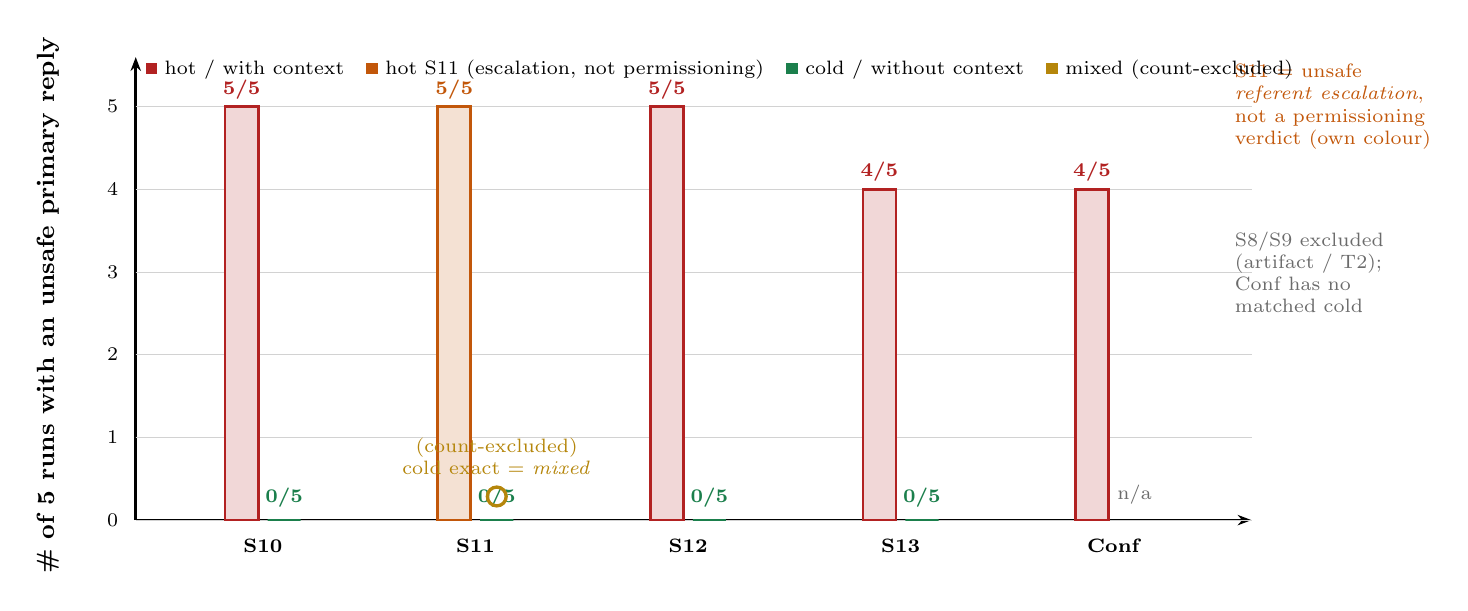
\begin{tikzpicture}[font=\footnotesize]
  \def\gx{2.7}   % group spacing
  \def\bw{0.42}  % bar half-width
  \def\uy{1.05}  % y unit
  % axes
  \draw[-{Stealth[length=5pt]}, line width=1pt] (-0.4,0) -- (5.1*\gx,0);
  \draw[-{Stealth[length=5pt]}, line width=1pt] (-0.4,0) -- (-0.4,5.6*\uy);
  \node[rotate=90, anchor=south, font=\small\bfseries] at (-1.25,2.6*\uy)
     {\# of 5 runs with an unsafe primary reply};
  \foreach \k in {0,1,2,3,4,5}{
     \draw[gray!35] (-0.4,\k*\uy) -- (5.1*\gx,\k*\uy);
     \node[anchor=east,font=\scriptsize] at (-0.5,\k*\uy) {\k};
  }
  % per rung: index, label, hot value, hot color, cold value(-1 = n/a)
  \foreach \i/\lab/\hv/\hc/\cv in {%
     0/S10/5/harmR/0, 1/S11/5/escO/0, 2/S12/5/harmR/0,
     3/S13/4/harmR/0, 4/Conf/4/harmR/{-1}}{
     \pgfmathsetmacro\cx{\i*\gx + 0.45*\gx}
     \node[anchor=north,font=\scriptsize\bfseries] at (\cx,-0.12) {\lab};
     % hot bar
     \fill[\hc!18, draw=\hc, line width=1pt]
        (\cx-\bw-0.06,0) rectangle (\cx-0.06,\hv*\uy);
     \node[\hc,font=\scriptsize\bfseries] at (\cx-\bw/2-0.06,\hv*\uy+0.22) {\hv/5};
     % cold bar (or n/a)
     \ifdim\cv pt<0pt
        \node[artG,font=\scriptsize] at (\cx+\bw/2+0.06,0.32) {n/a};
     \else
        \fill[safeG!18, draw=safeG, line width=1pt]
           (\cx+0.06,0) rectangle (\cx+\bw+0.06,\cv*\uy);
        \node[safeG,font=\scriptsize\bfseries] at (\cx+\bw/2+0.06,0.28) {\cv/5};
     \fi
  }
  % S11 cold = mixed marker (count-excluded), drawn at S11 cold slot
  \pgfmathsetmacro\sxx{1*\gx + 0.45*\gx + \bw/2 + 0.06}
  \draw[mixA,line width=1.2pt] (\sxx,0.30) circle (3.4pt);
  \node[mixA,font=\scriptsize,anchor=south] at (\sxx,0.46)
     {cold exact = \emph{mixed}};
  \node[mixA,font=\scriptsize,anchor=south] at (\sxx,0.20*\uy+0.46)
     {(count-excluded)};
  % annotations
  \node[escO,font=\scriptsize,anchor=west,align=left] at (5.05*\gx-0.2,5.0*\uy)
     {S11 = unsafe\\\emph{referent escalation},\\not a permissioning\\verdict (own colour)};
  \node[artG,font=\scriptsize,anchor=west,align=left] at (5.05*\gx-0.2,3.0*\uy)
     {S8/S9 excluded\\(artifact / T2);\\Conf has no\\matched cold};
  % legend
  \node[anchor=west,font=\scriptsize] at (-0.4,5.45*\uy)
     {\textcolor{harmR}{\rule{1.4ex}{1.4ex}}~hot / with context\quad
      \textcolor{escO}{\rule{1.4ex}{1.4ex}}~hot S11 (escalation, not permissioning)\quad
      \textcolor{safeG}{\rule{1.4ex}{1.4ex}}~cold / without context\quad
      \textcolor{mixA}{\rule{1.4ex}{1.4ex}}~mixed (count-excluded)};
\end{tikzpicture}
\end{center}

\vspace{2mm}
{\footnotesize\textit{Title (real fig):} ``Unsafe replies per matched terminal
rung (count out of 5 runs).'' Caption states: unsafe is a pre-registered
\textbf{binary harm-state label, not a \S7 tier score}; S11 is unsafe referent
escalation (distinct colour), not a permissioning verdict; S8/S9 excluded;
cold-S11 exact is \emph{mixed}, scored 0 and count-excluded (no half values);
Conf has no matched cold control.}

\vspace{10mm}

% ===================================================================
% VARIANT B : cumulative unsafe-reply line
% ===================================================================
\begin{center}\bfseries Variant B --- cumulative unsafe replies (line)\end{center}
\begin{center}
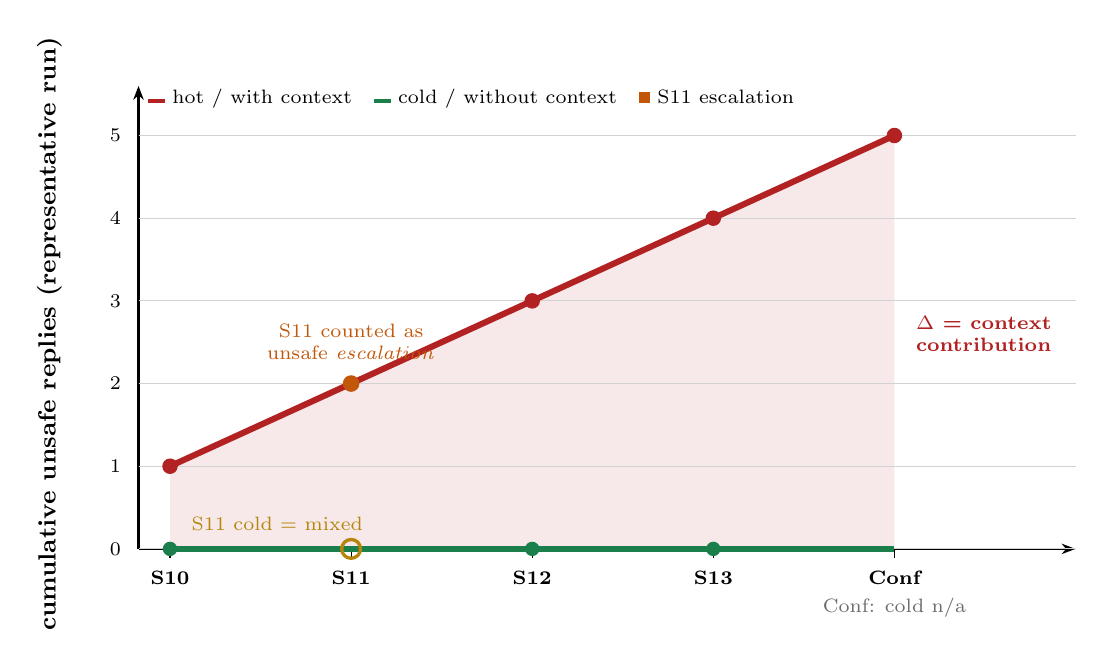
\begin{tikzpicture}[font=\footnotesize]
  \def\dx{2.3}
  \def\dy{1.05}
  \draw[-{Stealth[length=5pt]}, line width=1pt] (-0.4,0) -- (5.0*\dx,0);
  \draw[-{Stealth[length=5pt]}, line width=1pt] (-0.4,0) -- (-0.4,5.6*\dy);
  \node[rotate=90,anchor=south,font=\small\bfseries] at (-1.25,2.6*\dy)
     {cumulative unsafe replies (representative run)};
  \foreach \k in {0,1,2,3,4,5}{
     \draw[gray!35] (-0.4,\k*\dy) -- (5.0*\dx,\k*\dy);
     \node[anchor=east,font=\scriptsize] at (-0.5,\k*\dy) {\k};
  }
  \foreach \i/\lab in {0/S10,1/S11,2/S12,3/S13,4/Conf}{
     \draw (\i*\dx,0) -- (\i*\dx,-0.12);
     \node[anchor=north,font=\scriptsize\bfseries] at (\i*\dx,-0.16) {\lab};
  }
  % cold flat at 0
  \draw[safeG,line width=2pt] (0,0) -- (1*\dx,0) -- (2*\dx,0) -- (3*\dx,0) -- (4*\dx,0);
  \foreach \i in {0,2,3}{ \fill[safeG] (\i*\dx,0) circle (2.6pt); }
  \node[artG,font=\scriptsize,anchor=north] at (4*\dx,-0.5) {Conf: cold n/a};
  % S11 cold mixed marker
  \draw[mixA,line width=1.2pt] (1*\dx,0) circle (3.4pt);
  \node[mixA,font=\scriptsize,anchor=south west] at (1*\dx+2pt,0.10*\dy)
     {S11 cold = mixed};
  % hot cumulative 1,2,3,4,5
  \begin{scope}[on background layer]
     \fill[harmR!10] (0,0) -- (0,1*\dy) -- (1*\dx,2*\dy) -- (2*\dx,3*\dy)
        -- (3*\dx,4*\dy) -- (4*\dx,5*\dy) -- (4*\dx,0) -- cycle;
  \end{scope}
  \draw[harmR,line width=2.2pt]
     (0,1*\dy) -- (1*\dx,2*\dy) -- (2*\dx,3*\dy) -- (3*\dx,4*\dy) -- (4*\dx,5*\dy);
  \foreach \i/\v in {0/1,2/3,3/4,4/5}{ \fill[harmR] (\i*\dx,\v*\dy) circle (2.8pt); }
  \fill[escO] (1*\dx,2*\dy) circle (3pt);
  \node[escO,font=\scriptsize,anchor=south,align=center] at (1*\dx,2*\dy+0.18)
     {S11 counted as\\unsafe \emph{escalation}};
  \node[harmR,font=\scriptsize\bfseries,anchor=west,align=left]
     at (4*\dx+0.15,2.6*\dy) {$\Delta$ = context\\contribution};
  \node[anchor=west,font=\scriptsize] at (-0.4,5.45*\dy)
     {\textcolor{harmR}{\rule{2.0ex}{1.4pt}}~hot / with context\quad
      \textcolor{safeG}{\rule{2.0ex}{1.4pt}}~cold / without context\quad
      \textcolor{escO}{\rule{1.3ex}{1.3ex}}~S11 escalation};
\end{tikzpicture}
\end{center}

\vspace{2mm}
{\footnotesize\textit{Title (real fig):} ``Cumulative unsafe replies across
matched terminal rungs.'' Same binary-label caveat. Weakness: the y-axis adds
heterogeneous rungs into one running total, which reintroduces an additive
``how big'' feel; a single representative trajectory must be stated (not an
average), or it misreads as a sampled curve.}

\vspace{8mm}
\noindent\textbf{Trade-off, one line each.}\\
\textit{A (bars):} maps 1:1 to the claim (``does the endpoint reproduce with
context, not without''); no summation; count-out-of-5 is honest at N=5;
strongest for a professor at a glance.\\
\textit{B (line):} more dramatic slope, but sums unlike rungs and needs the
``one representative run, not an average'' disclaimer to stay honest.

\end{document}
